\documentclass[11pt]{article}
\usepackage[margin=1in]{geometry}
\usepackage[T1]{fontenc}
\usepackage{lmodern}
\usepackage{graphicx}
\usepackage{booktabs}
\usepackage{array}
\usepackage{float}
\usepackage{amsmath}
\usepackage{hyperref}
\usepackage{xcolor}

\hypersetup{
  colorlinks=true,
  linkcolor=blue,
  urlcolor=blue
}

\setlength{\parskip}{0.5em}
\setlength{\parindent}{0pt}

\title{Integrated Report for Implemented Task 3, Task 4, and Task 5 Components}
\author{}
\date{March 12, 2026}

\begin{document}
\maketitle

\section{Scope, Sources, and Bundle Structure}

This report consolidates the implemented scope from Task 3, Task 4, and Task 5 into
one folder under \texttt{Task5/report\_bundle}. The report is based on:
\begin{itemize}
  \item the case PDF requirements for Tasks 3, 4, and 5;
  \item the saved notebooks in \texttt{Task3}, \texttt{Task4}, and \texttt{Task5};
  \item the saved CSV, Parquet, and PNG artifacts already on disk;
  \item the Task 5 maintenance notes in \texttt{CONTEXT.md}, \texttt{PLAN.md}, and
  \texttt{ACTIVE\_FIXES.md}.
\end{itemize}

No model recomputation was performed for this report. Only saved artifacts were read,
summarized, copied, and packaged.

The bundle now contains:
\begin{itemize}
  \item this report as \texttt{task5\_report.tex} and \texttt{task5\_report.pdf};
  \item a \texttt{data/} folder with the supporting Task 3, Task 4, and Task 5 files used here;
  \item a \texttt{plots/} folder with the saved Task 3 figures and the copied Task 5 figures,
  plus Task 4 summary plots derived from the saved parquet output.
\end{itemize}

\textbf{Removed problematic files.} The documented problematic Task 5.9 detail files were
removed from the bundle:
\begin{itemize}
  \item \texttt{subtask\_5\_9\_cost\_carbon\_summary.csv};
  \item \texttt{lane\_cost\_carbon\_2030.csv};
  \item the stale 5.9 plots derived from those files.
\end{itemize}

For Task 5.9, the authoritative saved source in this report is
\texttt{data/network\_kpis\_by\_year.csv}, because that file contains the corrected
delivered-unit transport KPIs. The removed detail files were flagged in
\texttt{ACTIVE\_FIXES.md} as problematic.

\section{Task 3: Production Planning and Feasibility Scope}

\subsection{PDF Alignment}

The implemented Task 3 scope in this repository covers:
\begin{itemize}
  \item \textbf{Task 3.1}: estimate 99\%-robust steady daily production rates by product cluster and
  compute how early production must start before January 1 to maintain 12-week autonomy;
  \item \textbf{Task 3.2}: provide a production-feasibility simulator that validates inventory dynamics
  under those production rates.
\end{itemize}

The repository does \emph{not} include completed implementations for the Task 3.3 pallet
layout work or the Task 3.4 truck and tractor-trailer fleet sizing work.

\subsection{Task 3.1 Method}

The production notebook groups models into the two PDF-defined clusters:
\begin{itemize}
  \item Cluster 1: Floor Care, Kitchen Help, Leisure;
  \item Cluster 2: Safety \& Security, Wall \& Window Care, Exterior Care.
\end{itemize}

The method is:
\begin{enumerate}
  \item load all Task 2 demand simulation batches;
  \item aggregate annual sales by year, simulation, and cluster;
  \item compute the 99th percentile annual demand for each cluster-year;
  \item divide by 354 workdays per year to get the steady 99\%-robust daily production rate;
  \item compute the rolling 84-day forward demand requirement over the whole year;
  \item locate the critical date with maximum 84-day inventory stress;
  \item compute the required January 1 inventory and convert that requirement into prior start days.
\end{enumerate}

The key formulas are:
\[
\text{Daily Production}_{99\%} =
\frac{\text{Annual Demand P99}}{354}
\]

\[
\text{Required Inventory on Jan 1} =
\text{Max 84-day Autonomy Requirement} -
\text{Net Accumulation from Jan 1 to Critical Date}
\]

\subsection{Task 3.1 Results}

Production requirements grow substantially with market rollout. Cluster 1 rises from
47.88 units/day in 2027 to 558.06 units/day in 2034, while Cluster 2 rises from
35.31 units/day to 408.47 units/day over the same horizon.

\begin{table}[H]
\centering
\small
\begin{tabular}{rrrr}
\toprule
Year & Cluster & Daily production at 99\% robustness & Buffer over mean demand \% \\
\midrule
2027 & Cluster 1 & 47.88 & 3.80 \\
2027 & Cluster 2 & 35.31 & 5.65 \\
2030 & Cluster 1 & 360.51 & 3.46 \\
2030 & Cluster 2 & 265.52 & 5.90 \\
2034 & Cluster 1 & 558.06 & 4.75 \\
2034 & Cluster 2 & 408.47 & 6.00 \\
\bottomrule
\end{tabular}
\caption{Saved Task 3.1 production-rate outputs from \texttt{cluster\_production\_rates.csv}.}
\end{table}

The prior-start calculation shows that the system needs a long prebuild phase in the
early years, then stabilizes around roughly 97--120 days before year start by the
later years.

\begin{table}[H]
\centering
\small
\begin{tabular}{rrrrr}
\toprule
Year & Cluster & Critical date & Prior start days & Required Jan 1 inventory \\
\midrule
2027 & Cluster 1 & 2027-11-26 & 171 & 7,917 \\
2027 & Cluster 2 & 2027-11-26 & 157 & 5,354 \\
2030 & Cluster 1 & 2030-10-09 & 120 & 41,731 \\
2030 & Cluster 2 & 2030-11-22 & 118 & 30,140 \\
2034 & Cluster 1 & 2034-10-09 & 109 & 58,969 \\
2034 & Cluster 2 & 2034-10-09 & 114 & 45,150 \\
\bottomrule
\end{tabular}
\caption{Saved Task 3.1 prior-start outputs from \texttt{prior\_start\_days\_corrected.csv}.}
\end{table}

\begin{figure}[H]
\centering
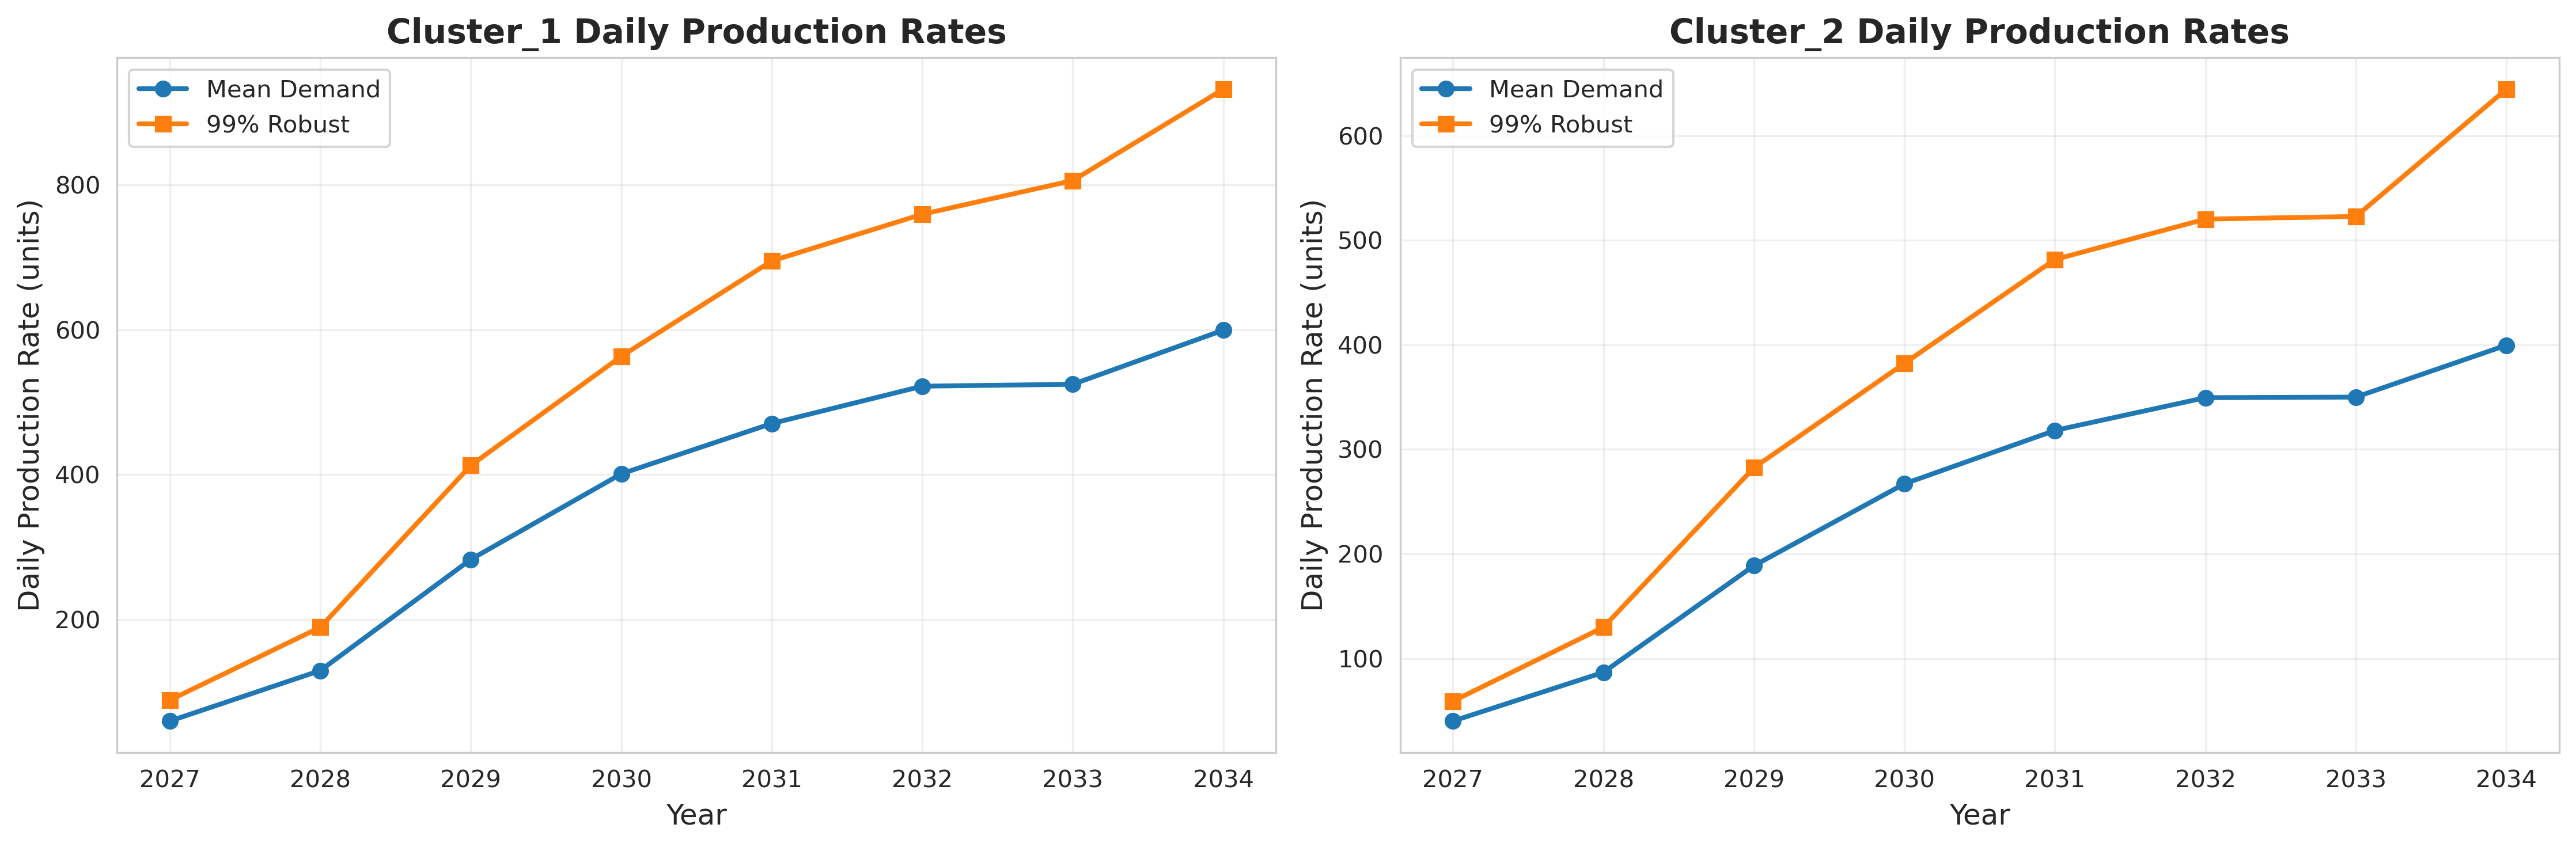
\includegraphics[width=0.82\textwidth]{plots/daily_production_rates.png}
\caption{Saved Task 3.1 daily production rate plot by cluster and year.}
\end{figure}

\begin{figure}[H]
\centering
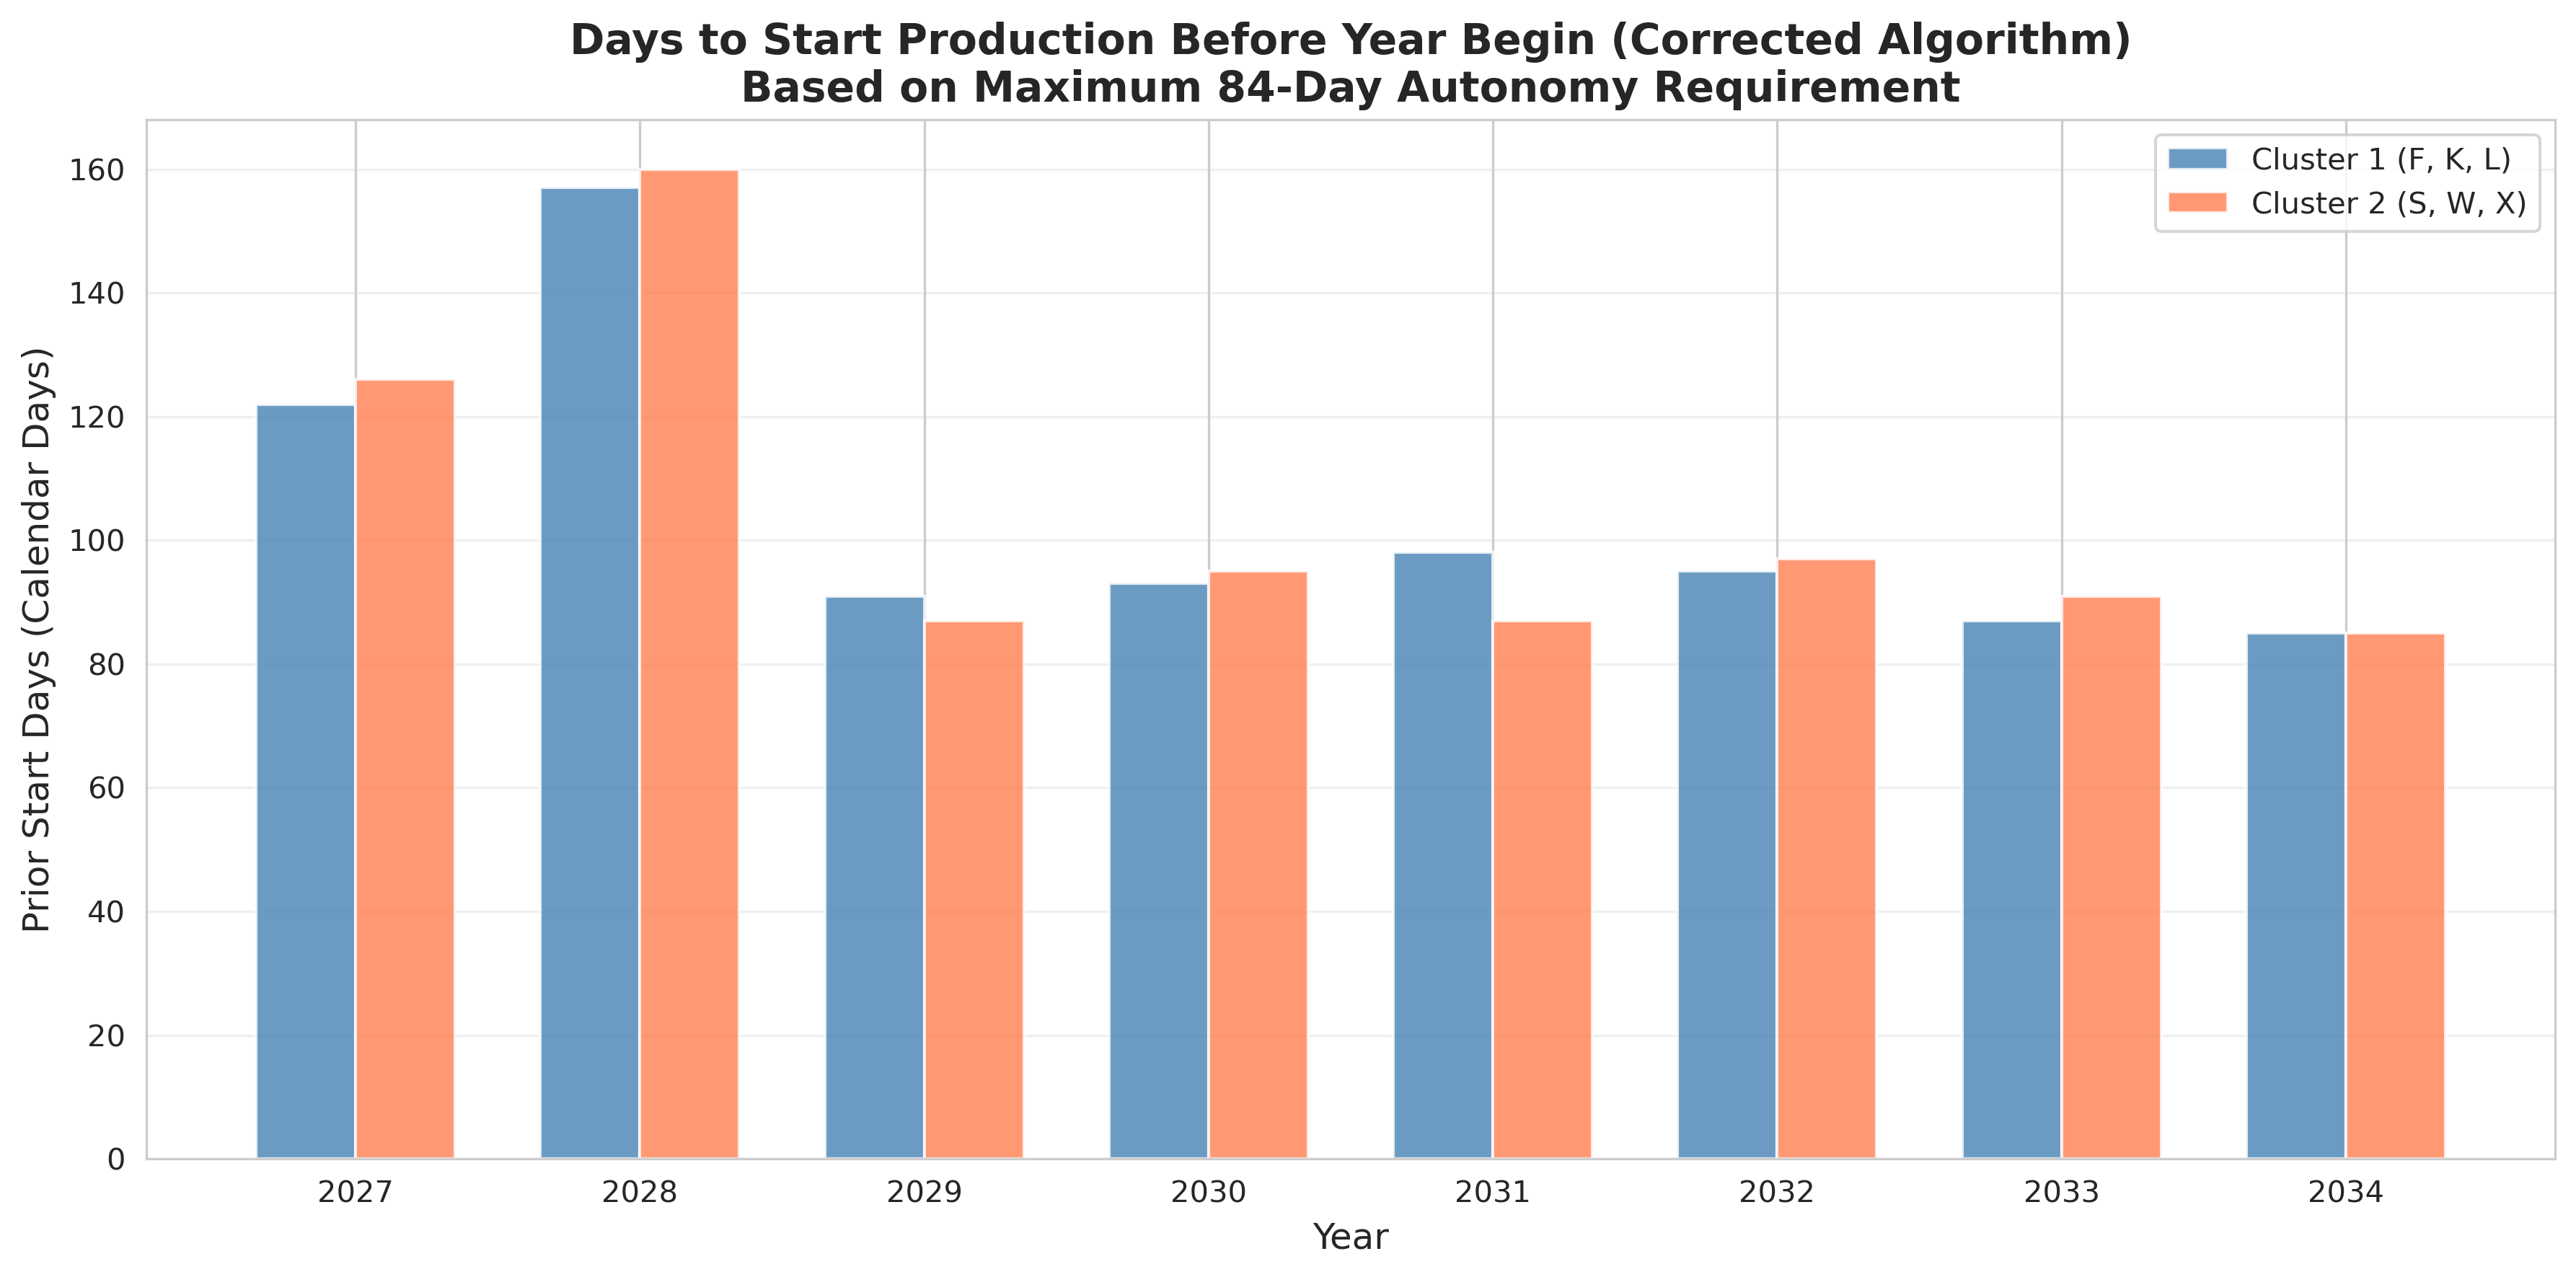
\includegraphics[width=0.78\textwidth]{plots/prior_start_days_corrected.png}
\caption{Saved Task 3.1 prior-start-days plot.}
\end{figure}

\begin{figure}[H]
\centering
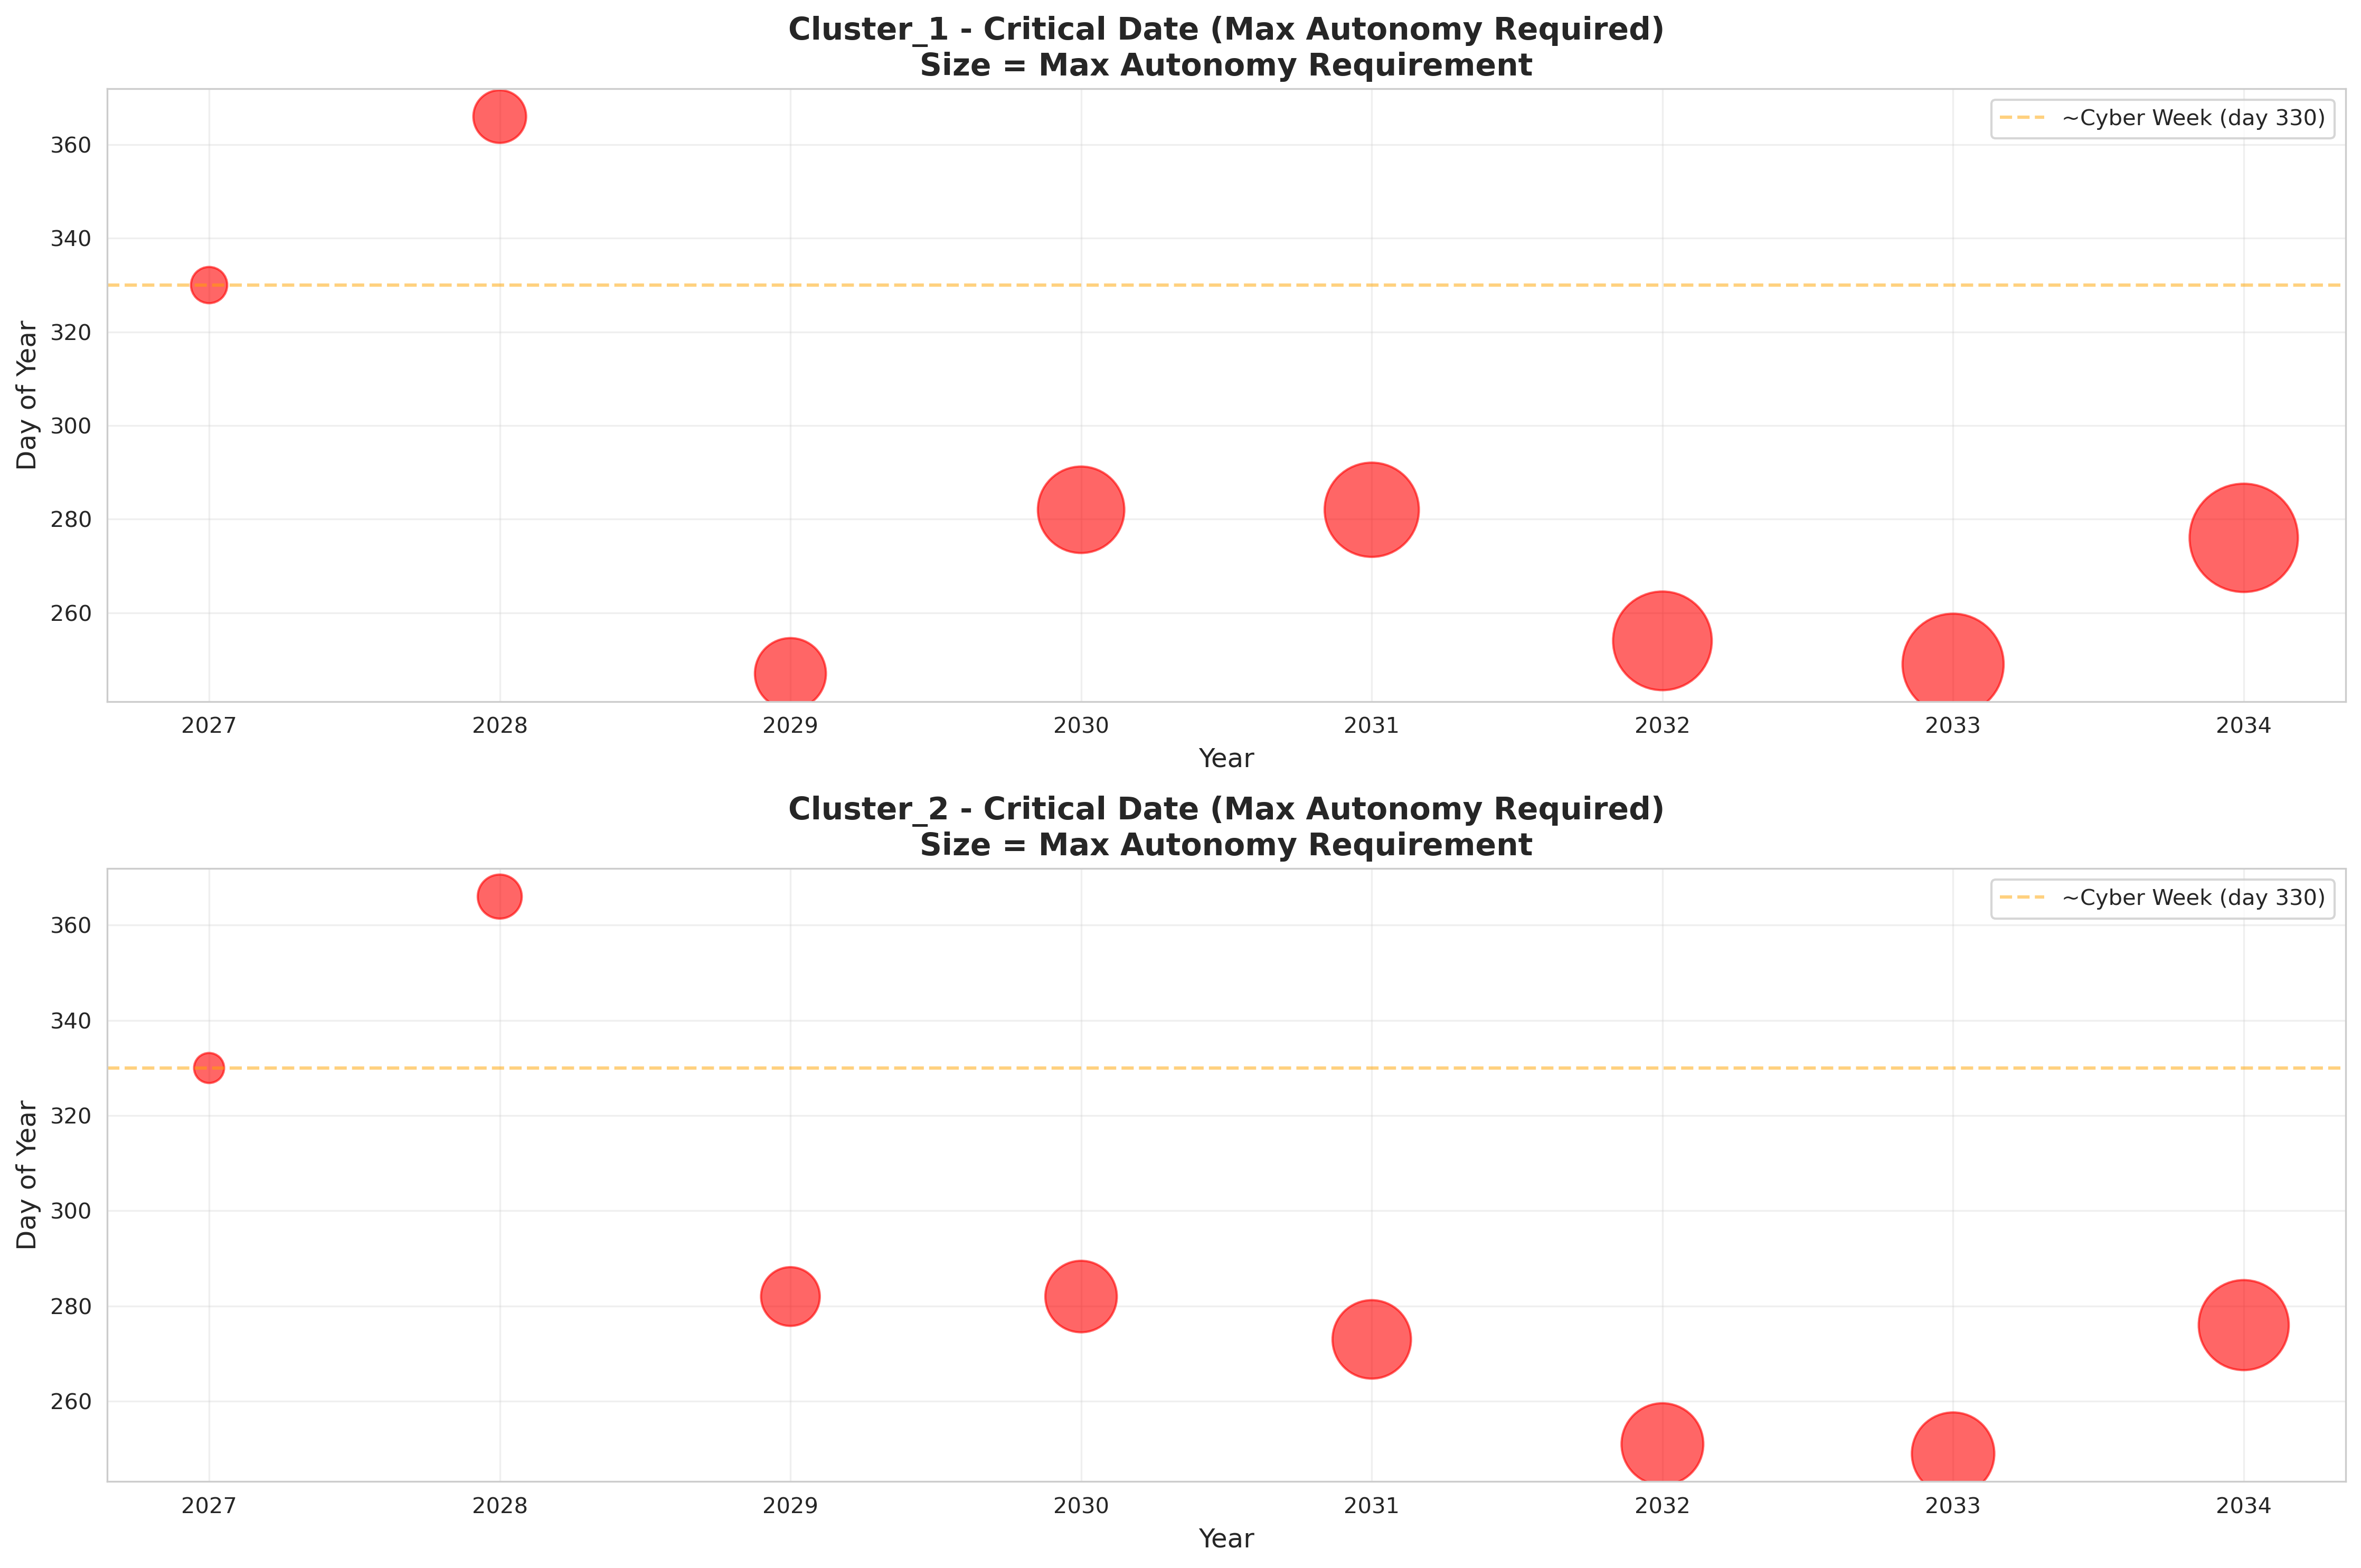
\includegraphics[width=0.82\textwidth]{plots/critical_dates_analysis.png}
\caption{Saved Task 3.1 critical-date analysis. Larger markers indicate larger maximum 84-day autonomy requirements.}
\end{figure}

\subsection{Task 3.2 Feasibility Simulator}

The repository also includes a \texttt{Production\_feasibility\_simulator.ipynb} notebook
for Task 3.2. Its daily logic is:
\[
\text{Inventory}_{t+1} =
\text{Inventory}_{t} + \text{Production}_{t} - \text{Demand}_{t}.
\]

For each simulation and cluster, the notebook:
\begin{itemize}
  \item starts production at the prior-start date from Task 3.1;
  \item produces at the steady daily 99\%-robust rate on modeled workdays;
  \item tracks daily inventory and 84-day forward demand;
  \item checks whether inventory covers the next 84 days of demand.
\end{itemize}

However, the repository does not include a saved validation CSV from a completed Task 3.2
run in the packaged artifacts. The implemented simulator logic is present and reportable,
but the persisted quantitative result set is limited to the Task 3.1 production and
prior-start outputs.

\begin{figure}[H]
\centering
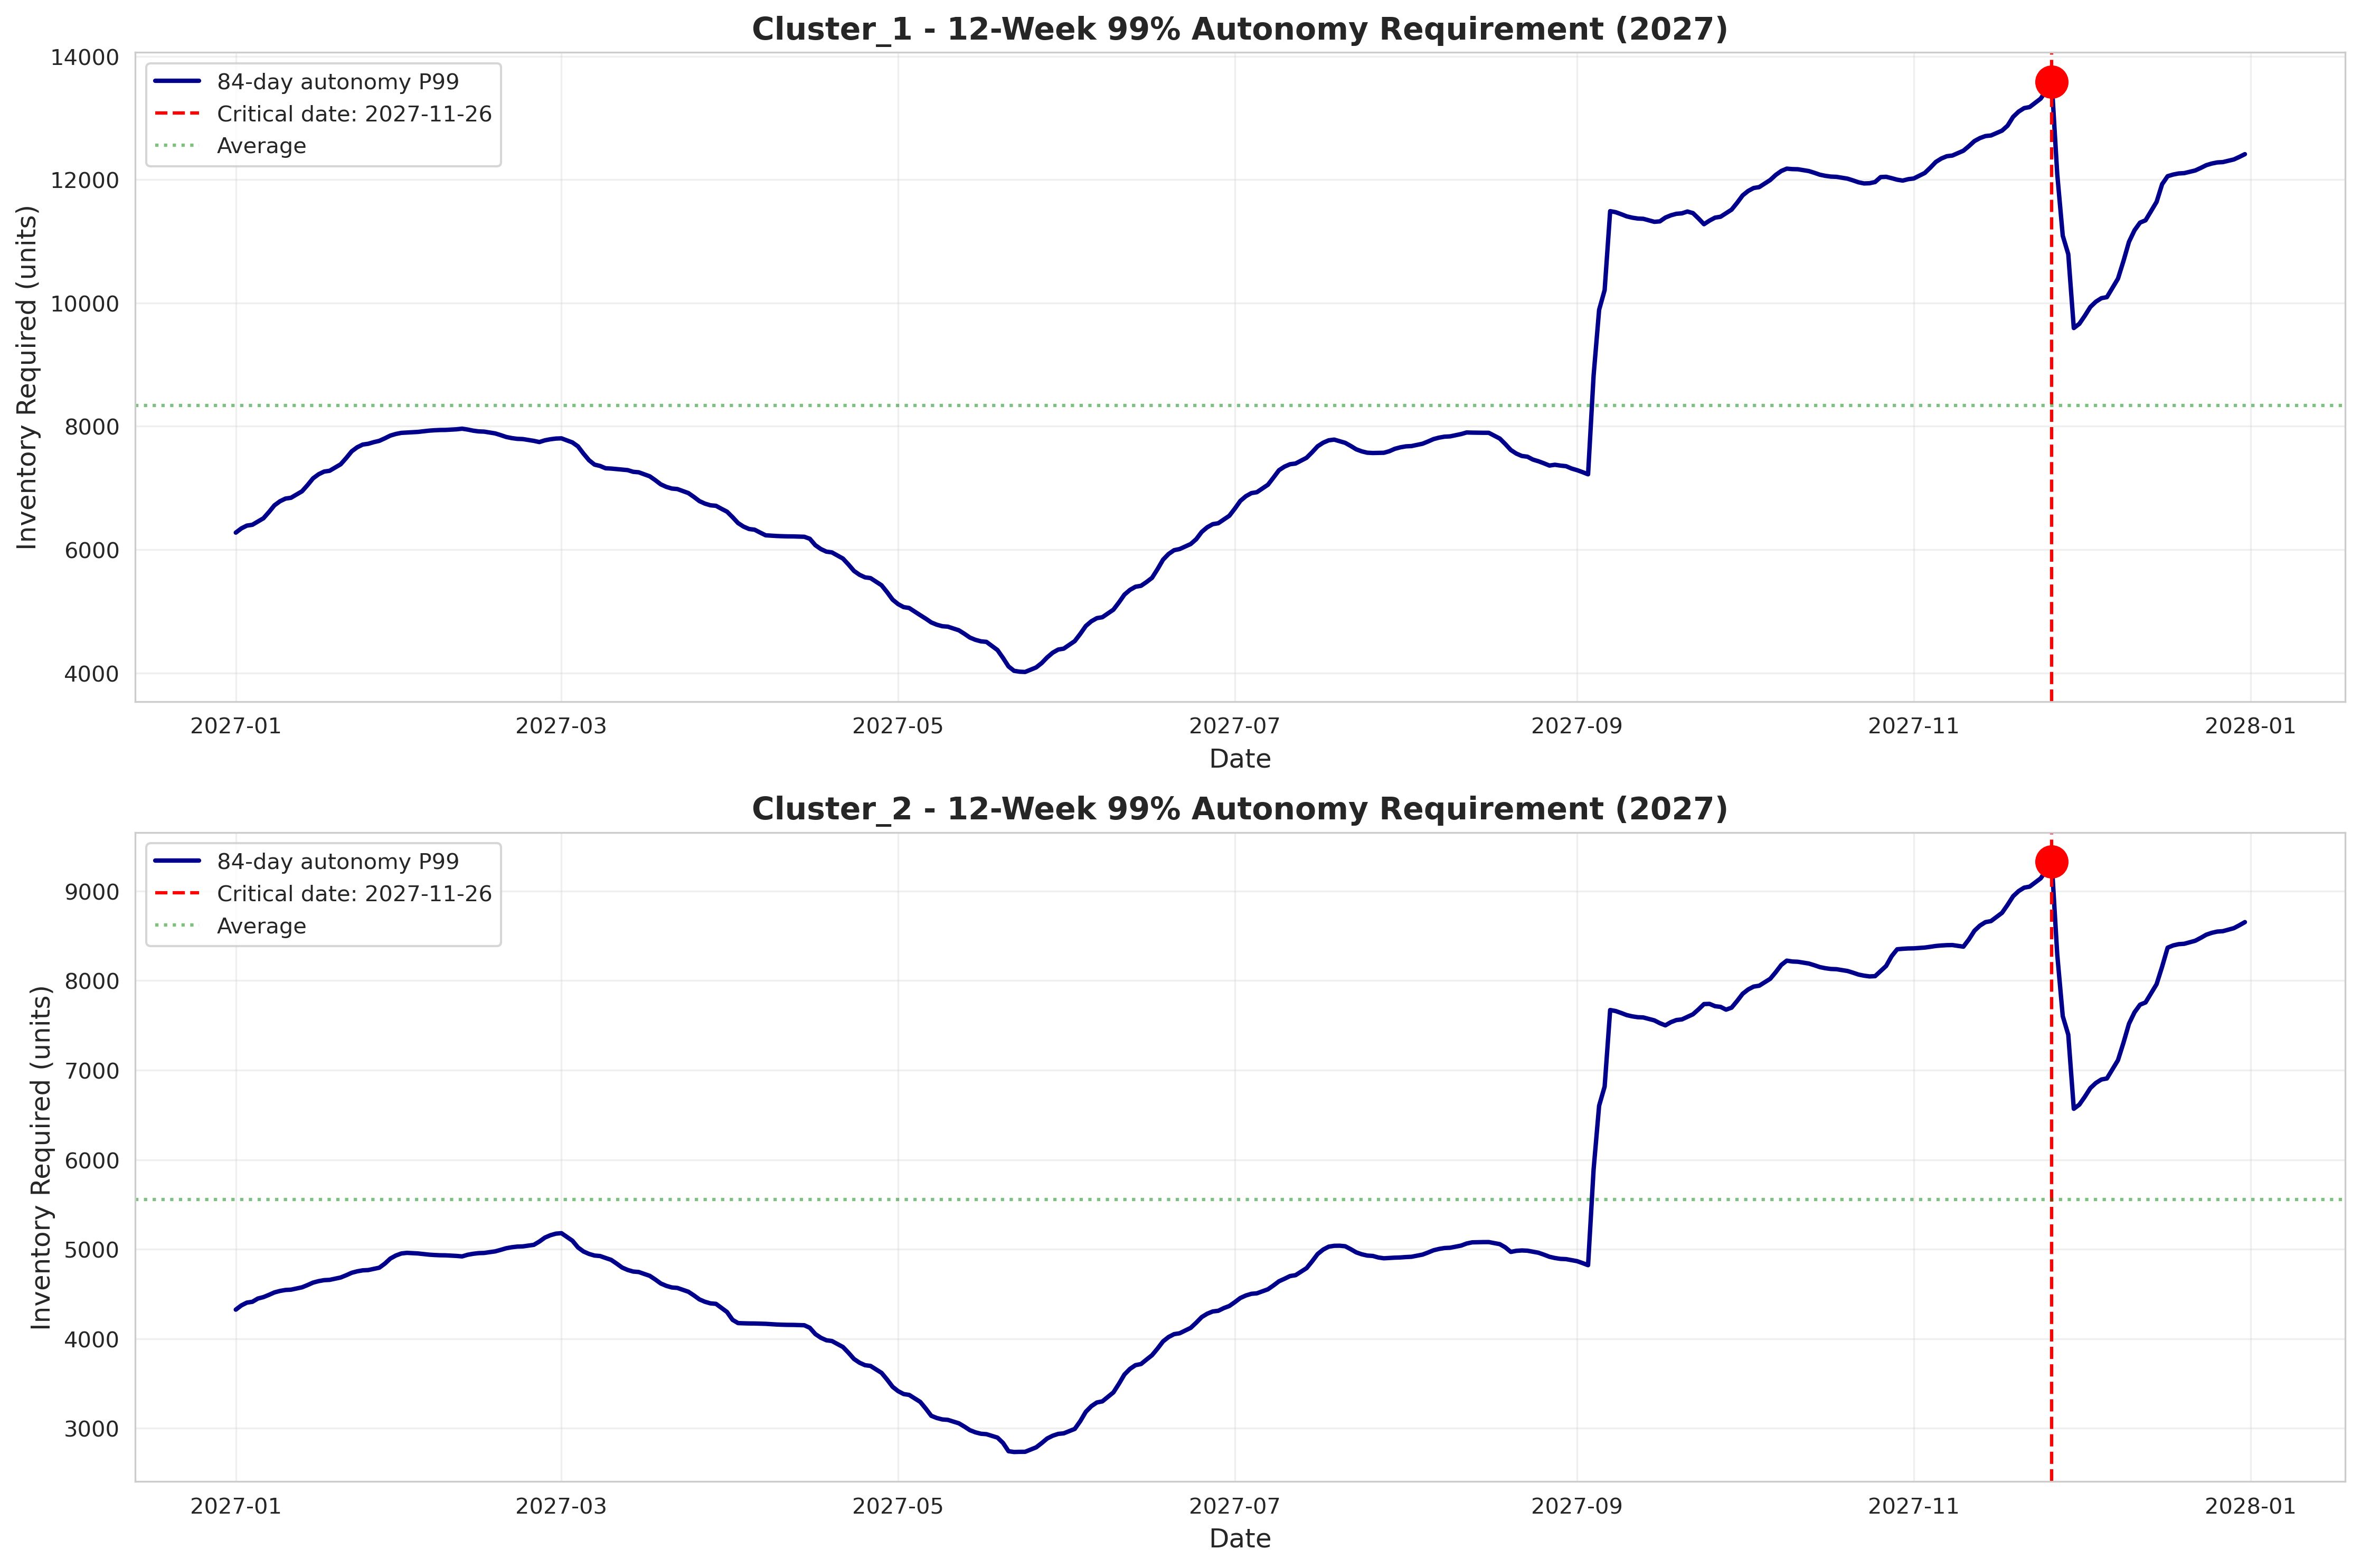
\includegraphics[width=0.82\textwidth]{plots/autonomy_inventory_2027_corrected.png}
\caption{Saved Task 3.1 autonomy-inventory profile for 2027, used as the basis for prior-start sizing.}
\end{figure}

\section{Task 4: DC-Level Demand Simulator Scope}

\subsection{PDF Alignment}

The implemented Task 4 scope in this repository is a \textbf{DC-level daily realized demand
simulator}. It supports the daily demand side of Task 4, especially the parts of the PDF that
require daily sales and outbound shipment modeling from Euro DCs. It does \emph{not} implement
the full container, ship, chassis, inventory-by-site, or fleet dynamics requested across all
Task 4 subtasks.

\subsection{Method}

The Task 4 notebook preserves the Task 2 stochastic demand logic and pushes it to DC level in
four stages:
\begin{enumerate}
  \item simulate demand at the \texttt{(country, segment)} level;
  \item use population-based city proportions from Task 2 assignments;
  \item collapse those city proportions into \texttt{segment\_dc\_weights};
  \item route each segment-day-model demand quantity directly to Euro DCs through those weights.
\end{enumerate}

The final output schema is:
\[
(\texttt{sim}, \texttt{date}, \texttt{year}, \texttt{euro\_dc\_id}, \texttt{model}, \texttt{realized\_units}).
\]

This implementation is computationally significant because it avoids materializing the full
city-level intermediate table. Instead, it uses pre-aggregated segment-to-DC weights and writes
Parquet batches.

\subsection{Saved Output Characteristics}

The saved Task 4 run produced:
\begin{itemize}
  \item 100 simulations over 2027--2034;
  \item 20 product models;
  \item 4 Euro DCs;
  \item 10 batch parquet files plus one merged \texttt{dc\_daily\_demand.parquet};
  \item 18,992,000 final records with an 81.3\% fill rate versus the dense upper bound.
\end{itemize}

\begin{table}[H]
\centering
\small
\begin{tabular}{rr}
\toprule
Year & Average annual realized units per simulation \\
\midrule
2027 & 8,574 \\
2028 & 17,587 \\
2029 & 46,487 \\
2030 & 73,403 \\
2031 & 88,753 \\
2032 & 97,533 \\
2033 & 105,483 \\
2034 & 113,448 \\
\bottomrule
\end{tabular}
\caption{Saved Task 4 average annual DC demand by year from \texttt{dc\_daily\_demand.parquet}.}
\end{table}

\begin{figure}[H]
\centering
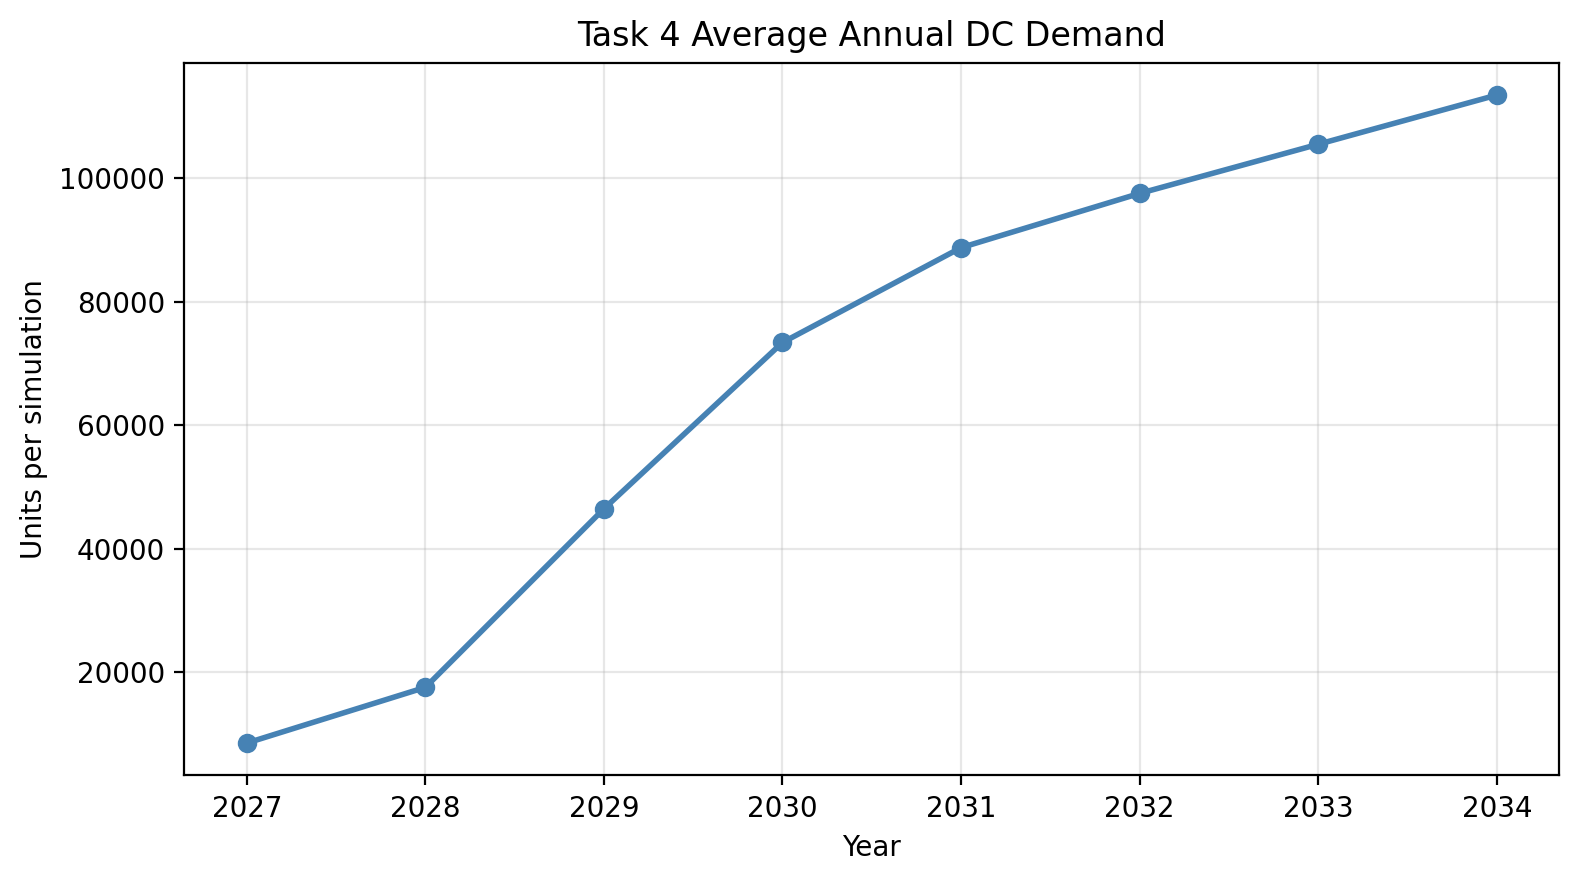
\includegraphics[width=0.78\textwidth]{plots/task4_annual_demand_by_year.png}
\caption{Task 4 annual realized demand trend derived from the saved parquet output.}
\end{figure}

By 2030 the saved DC split is already fully multi-DC, with Cologne still dominant but with
material demand also routed to Madrid, Rome, and Lodz.

\begin{table}[H]
\centering
\small
\begin{tabular}{lrr}
\toprule
Year & Euro DC & Average annual units per simulation \\
\midrule
2030 & CAND\_DE\_koeln & 27,163 \\
2030 & CAND\_ES\_madrid & 14,781 \\
2030 & CAND\_IT\_rome & 15,751 \\
2030 & CAND\_PL\_lodz & 15,707 \\
2034 & CAND\_DE\_koeln & 38,604 \\
2034 & CAND\_ES\_madrid & 22,835 \\
2034 & CAND\_IT\_rome & 26,926 \\
2034 & CAND\_PL\_lodz & 25,084 \\
\bottomrule
\end{tabular}
\caption{Saved Task 4 DC allocation pattern in later years.}
\end{table}

\begin{figure}[H]
\centering
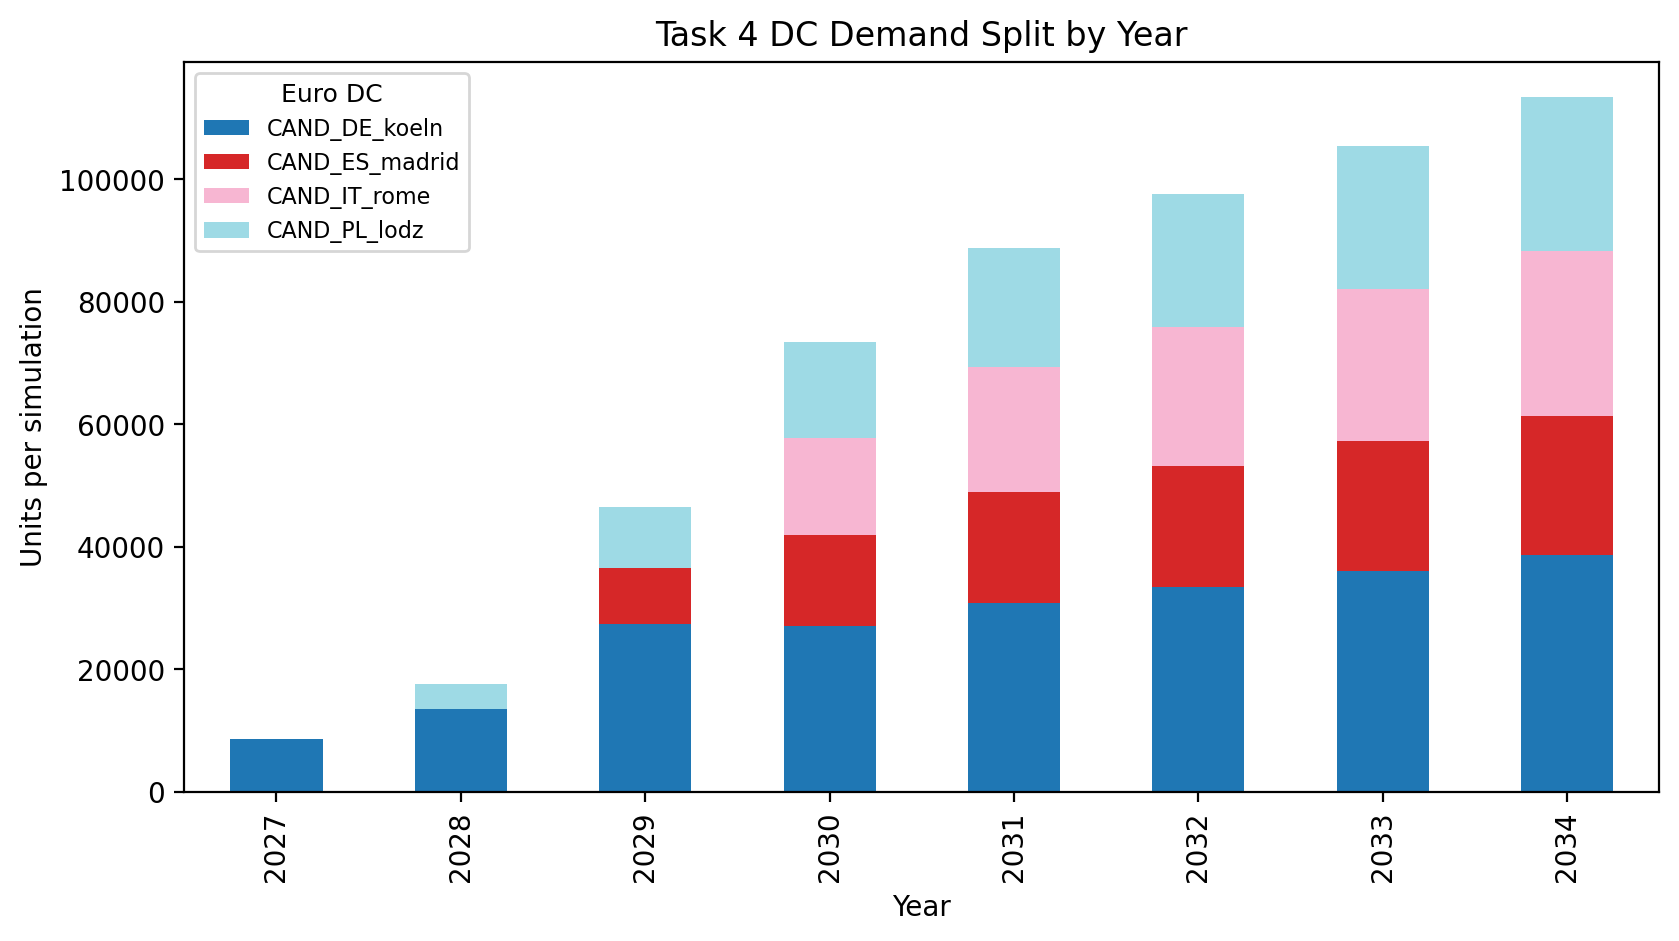
\includegraphics[width=0.82\textwidth]{plots/task4_dc_demand_by_year.png}
\caption{Task 4 DC demand mix by year derived from the saved parquet output.}
\end{figure}

Interpretation: the Task 4 artifact is best viewed as a clean daily DC-demand layer that feeds
later capacity, inventory, and network work. It is not yet a full Task 4 end-to-end operational
simulation of containers, tractors, chassis, ships, or site inventories.

\section{Task 5: Hyperconnected PI Network Scope}

\subsection{Implemented Coverage}

The saved Task 5 implementation covers the PI-network roadmap, PI packaging savings, route-backed
OTD, route-backed realized demand, a joint-shipment illustration, relay-readiness metrics, DC
sizing, transload cost, and PI profitability. The non-PI comparison requested in Task 5.14 is
not part of the current scope. Task 5.13 is only partially covered through saved CO$_2$ outputs;
there is no separate fuel or energy file in the bundle.

\subsection{Algorithms and Data Flow}

The Task 5 yearly pipeline runs from 2027 to 2034:
\begin{enumerate}
  \item activate yearly open-country nodes;
  \item derive relay hubs for paths exceeding the single-driver limit;
  \item generate physical lane legs;
  \item build shortest-elapsed-time DC-to-hub routes over those legs;
  \item build a service matrix that assigns each demand node to its best PI route;
  \item compute end-to-end PI OTD and purchase probability;
  \item simulate daily DC demand by model;
  \item size DC capacity and compute profitability.
\end{enumerate}

The key Task 5 data structures are:
\begin{itemize}
  \item \texttt{active\_nodes}: the yearly node roster after opening rules and relay derivation;
  \item \texttt{lanes}: physical legs such as \texttt{PORT\_DC}, \texttt{DC\_RELAY}, and
  \texttt{HUB\_CORRIDOR};
  \item \texttt{routes}: reconstructed multi-leg DC-to-hub paths with elapsed time and detour;
  \item \texttt{service\_matrix}: the node-level service view used for OTD and realized demand;
  \item \texttt{dc\_daily\_sim}: simulator-backed DC-model daily demand output;
  \item \texttt{kpis}: the final saved yearly KPI summary used in this report.
\end{itemize}

The Task 5 end-to-end PI OTD logic is:
\[
\text{OTD} = \text{route travel elapsed} + \text{PI last mile}.
\]

The saved PI last-mile assumptions follow the PDF:
\begin{itemize}
  \item metro: 4 h for 1M+, 2 h for 250K--1M, 1 h for less than 250K;
  \item non-metro: 8 h within 250 km, 16 h within 500 km, 32 h beyond 500 km.
\end{itemize}

\subsection{Task 5.1: Network Roadmap}

The network grows from one DC in 2027 to four DCs by 2030. Coverage remains above 97\%
throughout the rollout, and routed detour stays tightly controlled.

\begin{table}[H]
\centering
\small
\begin{tabular}{rrrrrrrr}
\toprule
Year & DCs & Peri hubs & Relay hubs & Lanes & Coverage \% & Relay ready \% & Mean detour \\
\midrule
2027 & 1 & 71 & 0 & 2,622 & 100.00 & 98.09 & 1.001 \\
2028 & 2 & 111 & 23 & 3,462 & 99.10 & 89.57 & 1.016 \\
2029 & 3 & 232 & 103 & 6,667 & 97.41 & 74.73 & 1.029 \\
2030 & 4 & 269 & 167 & 8,151 & 97.40 & 69.28 & 1.021 \\
2034 & 4 & 269 & 167 & 8,151 & 97.40 & 69.28 & 1.021 \\
\bottomrule
\end{tabular}
\caption{Saved Task 5 network KPIs from \texttt{network\_kpis\_by\_year.csv}.}
\end{table}

\begin{figure}[H]
\centering
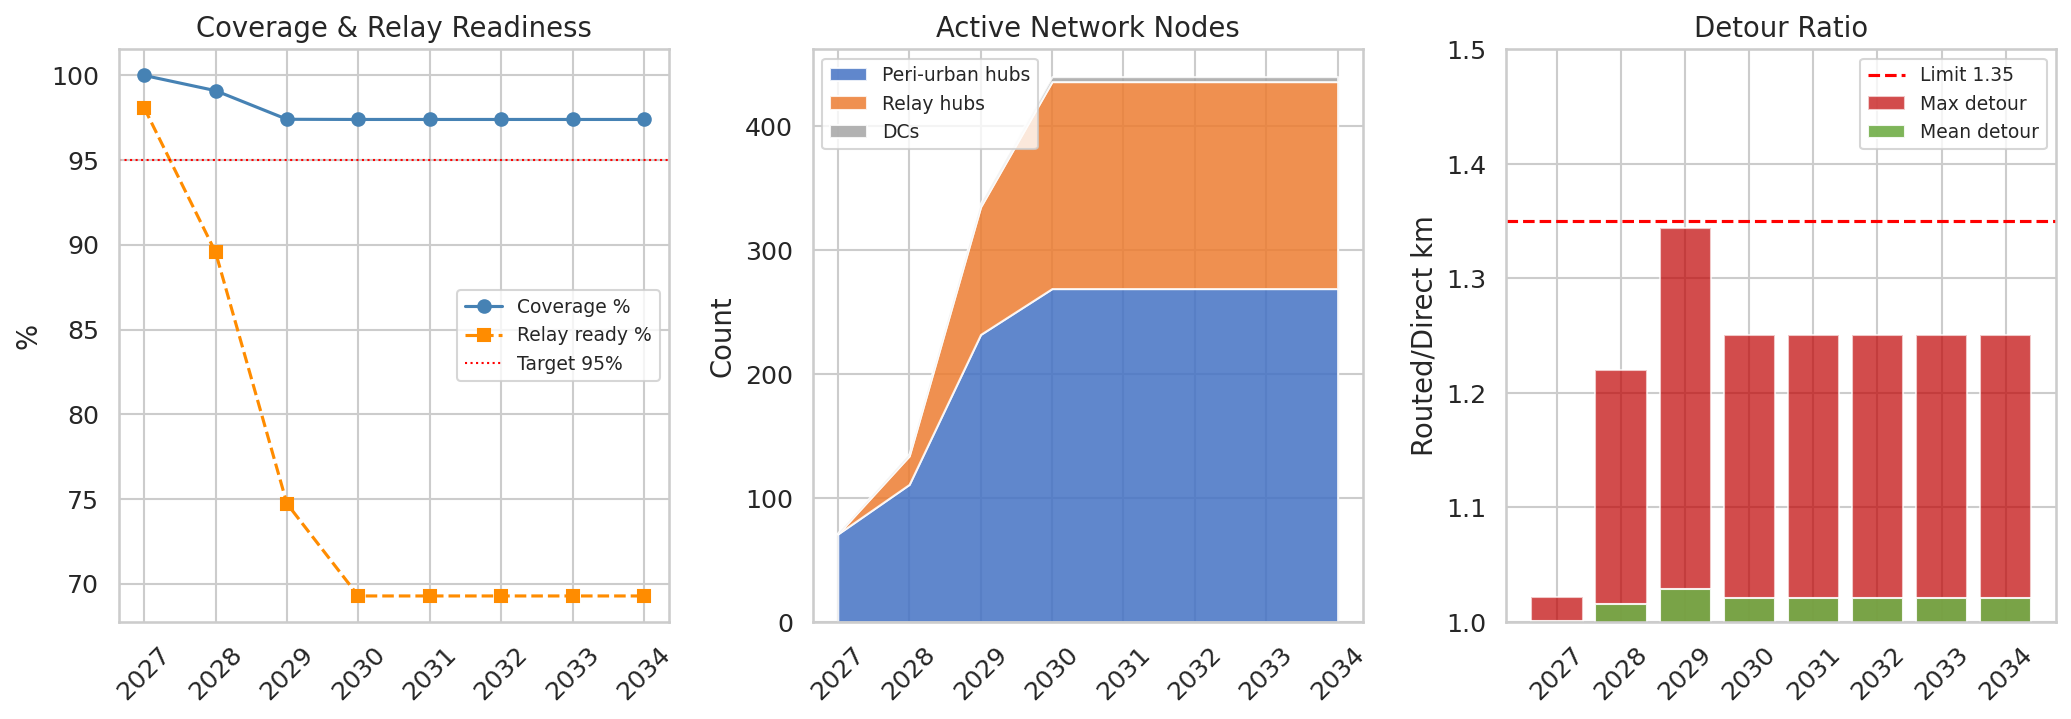
\includegraphics[width=0.82\textwidth]{plots/fig_5_1_topology_kpis.png}
\caption{Saved Task 5 network KPI trends.}
\end{figure}

\begin{figure}[H]
\centering

\includegraphics[width=0.82\textwidth]{plots/fig_5_1_network_map_2030.png}
\caption{Saved 2030 PI network map with the port, four Euro DCs, peri-urban hubs, and relay hubs.}
\end{figure}

The saved 2030 roadmap centers the four Euro DCs on Cologne, Lodz, Madrid, and Rome.
That produces a balanced west-central-east-south structure for the fully opened European market.

\subsection{Task 5.2: PI Packaging and Space Savings}

The saved packaging analysis shows stable structural savings:
\begin{itemize}
  \item 33.3\% fewer pallet positions;
  \item about 57.9\% fewer TEUs;
  \item annual packaging plus container savings growing from about EUR 0.87M in 2027
  to about EUR 10.16M in 2034.
\end{itemize}

\begin{table}[H]
\centering
\small
\begin{tabular}{rrrrrrr}
\toprule
Year & PI units & PI pallets & PI TEUs & Pallet saving \% & TEU saving \% & Total saving (EUR M) \\
\midrule
2027 & 28,602 & 4,767 & 157 & 33.3 & 57.8 & 0.87 \\
2030 & 218,466 & 36,411 & 1,194 & 33.3 & 57.9 & 6.62 \\
2034 & 335,412 & 55,902 & 1,833 & 33.3 & 57.9 & 10.16 \\
\bottomrule
\end{tabular}
\caption{Saved Task 5 PI packaging and container savings.}
\end{table}

\begin{figure}[H]
\centering
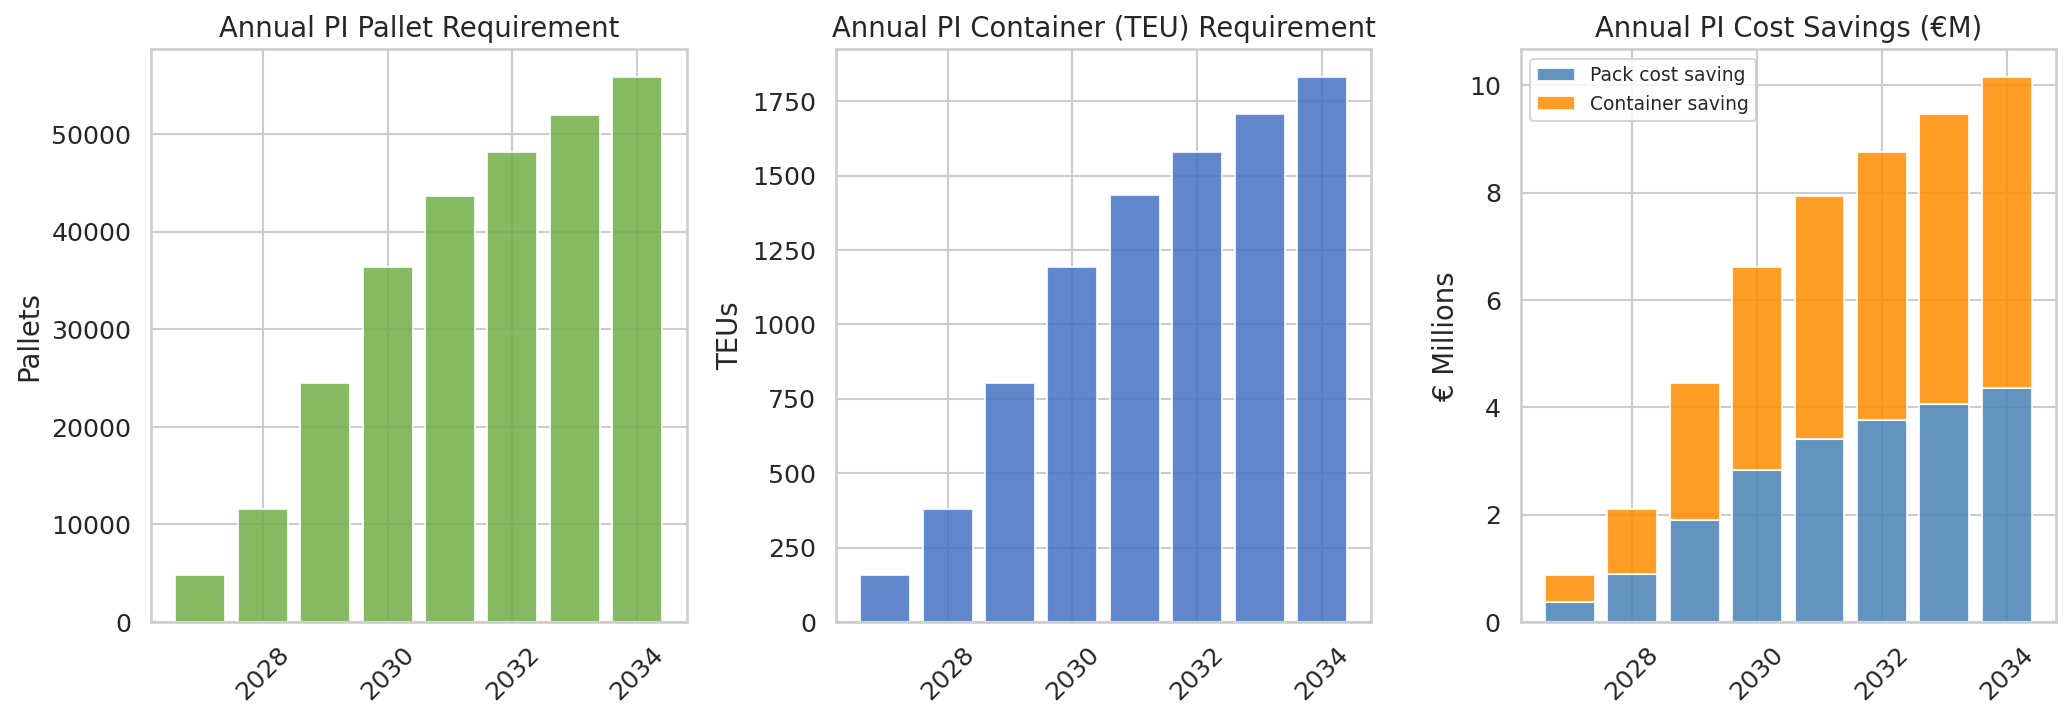
\includegraphics[width=0.82\textwidth]{plots/fig_5_2_container_savings.png}
\caption{Saved Task 5 PI packaging and container savings plot.}
\end{figure}

\subsection{Tasks 5.3 and 5.5: OTD and Realized PI Demand}

The saved OTD profile shows that the largest demand volume is still in the fast service classes.
The longest non-metro tail is the only segment with a substantial purchase-probability penalty.

\begin{table}[H]
\centering
\small
\begin{tabular}{lrrrrr}
\toprule
2030 service class & Nodes & Mean OTD (h) & P95 OTD (h) & Mean purchase prob. & Annual realized units \\
\midrule
METRO\_1M+ & 32 & 14.996 & 30.736 & 0.995 & 31,764.6 \\
METRO\_250K-1M & 127 & 10.029 & 19.797 & 0.999 & 28,386.2 \\
METRO\_<250K & 108 & 9.612 & 23.889 & 0.996 & 10,117.8 \\
METRO\_UNKNOWN & 6 & 1.000 & 1.000 & 1.000 & 6,233.8 \\
NONMETRO\_<=250KM & 23 & 16.442 & 21.951 & 0.999 & 130,773.7 \\
NONMETRO\_<=500KM & 3 & 31.866 & 34.407 & 0.980 & 7,185.1 \\
NONMETRO\_>500KM & 3 & 62.057 & 78.890 & 0.920 & 4,004.7 \\
\bottomrule
\end{tabular}
\caption{Saved 2030 Task 5 service-class OTD and realized demand summary.}
\end{table}

\begin{figure}[H]
\centering
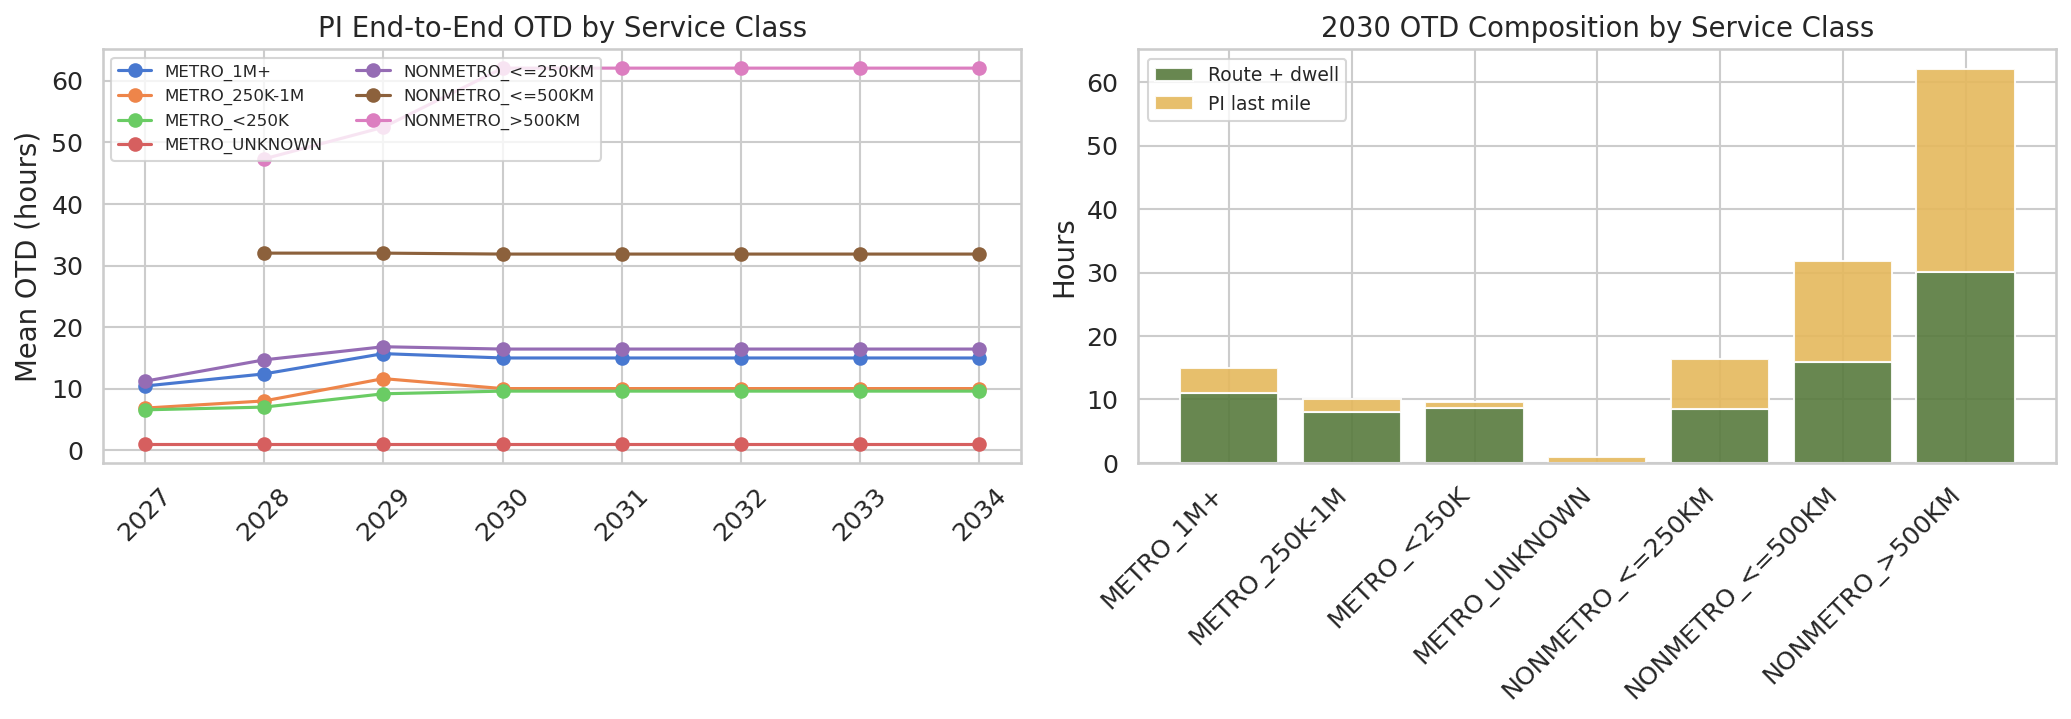
\includegraphics[width=0.82\textwidth]{plots/fig_5_3_otd_profile.png}
\caption{Saved Task 5 OTD profile by service class.}
\end{figure}

\begin{figure}[H]
\centering

\includegraphics[width=0.78\textwidth]{plots/fig_5_3_otd_distribution.png}
\caption{Saved Task 5 2030 OTD distribution by service class.}
\end{figure}

The saved PI demand summary grows from 28.6k units in 2027 to 335.4k units by 2034,
with route-backed coverage staying at about 97\% after the full four-DC rollout.

\begin{table}[H]
\centering
\small
\begin{tabular}{rrrrrr}
\toprule
Year & Realized PI units & PI revenue (EUR M) & Active service nodes & Route-backed nodes & Mean purchase prob. \\
\midrule
2027 & 28,602 & 12.97 & 76 & 76 & 1.0000 \\
2030 & 218,466 & 99.10 & 302 & 293 & 0.9966 \\
2034 & 335,411 & 152.14 & 302 & 293 & 0.9966 \\
\bottomrule
\end{tabular}
\caption{Saved Task 5 PI demand summary.}
\end{table}

\begin{figure}[H]
\centering

\includegraphics[width=0.82\textwidth]{plots/fig_5_5_demand_uplift.png}
\caption{Saved Task 5 realized PI demand and PI revenue trend.}
\end{figure}

\subsection{Task 5.4: Joint Shipment Illustration}

The saved illustrative shipment path is:
\[
\texttt{PORT\_NL\_rotterdam}
\rightarrow
\texttt{CAND\_DE\_koeln}
\rightarrow
\texttt{METRO\_BE\_brussels}.
\]

The saved cumulative elapsed time is 8.635 hours:
\begin{itemize}
  \item Rotterdam to Cologne: 203.6 km, 2.443 h drive, 2.0 h dwell;
  \item Cologne to Brussels: 182.7 km, 2.192 h drive, 2.0 h dwell.
\end{itemize}

\begin{figure}[H]
\centering

\includegraphics[width=0.78\textwidth]{plots/fig_5_4_joint_shipment.png}
\caption{Saved Task 5 joint-shipment trace.}
\end{figure}

\subsection{Task 5.6: Relay Readiness and Structural Autonomy}

The saved Task 5.6 output operationalizes autonomy structurally through relay-readiness
and dual-role-hub share rather than through explicit days-at-robustness targets.

\begin{table}[H]
\centering
\small
\begin{tabular}{rrrrr}
\toprule
Year & Relay readiness \% & DC-DC relay required \% & Dual-role hubs & Dual-role share \% \\
\midrule
2027 & 98.09 & 0.00 & 0 & 0.00 \\
2028 & 89.57 & 0.00 & 56 & 50.45 \\
2029 & 74.73 & 66.67 & 182 & 78.45 \\
2030 & 69.28 & 83.33 & 250 & 92.94 \\
2034 & 69.28 & 83.33 & 250 & 92.94 \\
\bottomrule
\end{tabular}
\caption{Saved Task 5.6 relay-readiness outputs.}
\end{table}

\begin{figure}[H]
\centering
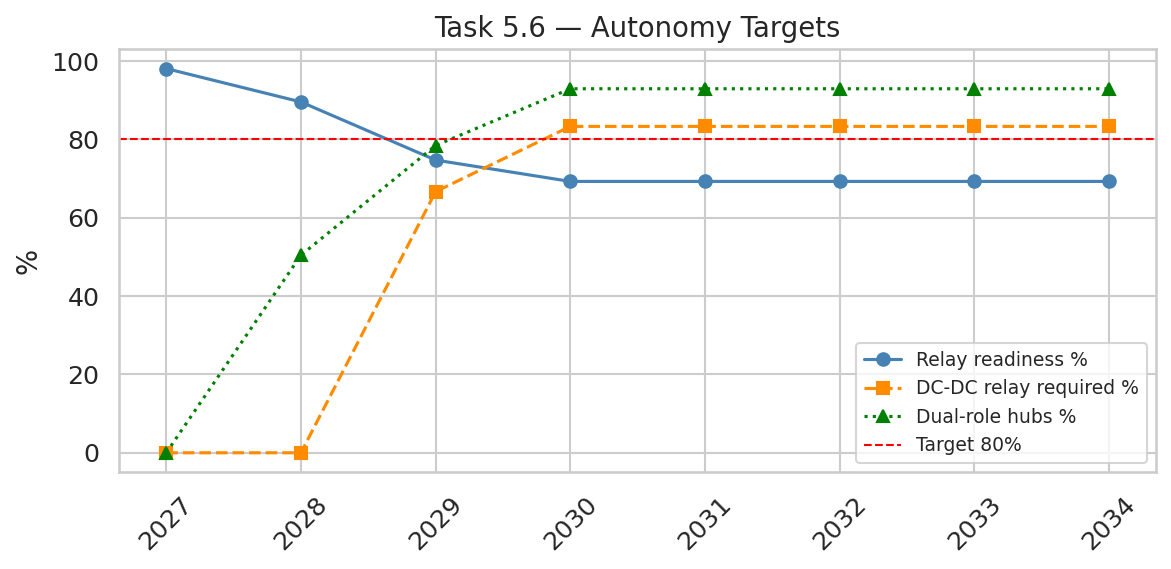
\includegraphics[width=0.72\textwidth]{plots/fig_5_6_autonomy.png}
\caption{Saved Task 5 relay-readiness and dual-role-hub trend.}
\end{figure}

\subsection{Tasks 5.9, 5.10, 5.11, and 5.12}

\textbf{Task 5.9.} Using the corrected saved KPI file, total transport cost rises from
EUR 0.76M in 2027 to EUR 24.36M in 2034. CO$_2$ rises from 245.6 tonnes to
11,202.8 tonnes, and the corrected delivered-unit transport cost increases from
EUR 26.63/unit to EUR 72.61/unit.

\textbf{Task 5.10.} The saved 2030 DC sizing output is concentrated in Cologne and Lodz.
Cologne carries the highest throughput requirement.

\begin{table}[H]
\centering
\small
\begin{tabular}{lrrrrr}
\toprule
2030 DC & Annual units & P95 peak daily units & Throughput cap & Storage positions & DC cost (EUR M) \\
\midrule
Cologne & 109,711 & 4,747 & 1,584 & 702 & 1.211 \\
Madrid & 22,305 & 965 & 322 & 143 & 0.724 \\
Rome & 34,545 & 1,495 & 500 & 221 & 0.792 \\
Lodz & 51,905 & 2,246 & 750 & 332 & 0.889 \\
\bottomrule
\end{tabular}
\caption{Saved Task 5 2030 DC sizing output.}
\end{table}

\begin{figure}[H]
\centering

\includegraphics[width=0.82\textwidth]{plots/fig_5_10_dc_capacity.png}
\caption{Saved Task 5 DC capacity and annual operating cost trend.}
\end{figure}

\textbf{Task 5.11.} Saved transload cost reaches EUR 655k in 2030 and EUR 1.01M in 2034.

\textbf{Task 5.12.} The saved PI-only profitability output remains strongly positive across all
years.

\begin{table}[H]
\centering
\small
\begin{tabular}{rrrrrr}
\toprule
Year & Transport cost (EUR M) & Total CO$_2$ (t) & Cost per unit (EUR) & PI margin (EUR M) & PI margin \% \\
\midrule
2027 & 0.76 & 245.6 & 26.628 & 10.73 & 82.73 \\
2030 & 15.13 & 6,901.2 & 69.261 & 75.00 & 75.69 \\
2034 & 24.36 & 11,202.8 & 72.614 & 115.31 & 75.79 \\
\bottomrule
\end{tabular}
\caption{Saved corrected Task 5 transport and profitability summary.}
\end{table}

\begin{figure}[H]
\centering

\includegraphics[width=0.82\textwidth]{plots/fig_5_12_profitability.png}
\caption{Saved Task 5 profitability trend.}
\end{figure}

\begin{figure}[H]
\centering

\includegraphics[width=0.82\textwidth]{plots/fig_5_12_pl_waterfall_2030.png}
\caption{Saved Task 5 2030 PI profit-and-loss waterfall.}
\end{figure}

\section{Discussion and Remaining Gaps}

Across the implemented scope, the repository tells a coherent story:
\begin{itemize}
  \item Task 3 provides a defensible production-rate and prior-start calculation for 12-week,
  99\% autonomy at the cluster level;
  \item Task 4 provides a scalable DC-level daily demand simulator that can feed later capacity
  and network work;
  \item Task 5 builds a route-backed PI network layer on top of that demand structure and
  produces credible PI-only packaging, OTD, demand, sizing, and profitability outputs.
\end{itemize}

The main limitations are:
\begin{itemize}
  \item Task 3.2 simulator logic exists, but the bundle does not contain a saved quantitative
  validation result set from a completed run;
  \item Task 4 does not yet implement the full container, ship, chassis, inventory-by-site, and
  fleet dynamics requested in the PDF;
  \item Task 5.6 is represented by relay-readiness metrics rather than explicit autonomy targets
  in days and robustness percent;
  \item Task 5.13 has CO$_2$ outputs but not a separate energy estimate;
  \item Task 5.14 and Task 5.15 are outside the current saved scope.
\end{itemize}

\section{Conclusion}

The saved repository artifacts are strongest as a staged analytical chain:
\begin{itemize}
  \item Task 3 converts uncertain demand into robust cluster-level production and launch timing;
  \item Task 4 converts market demand into DC-level daily realized demand;
  \item Task 5 converts that operational demand view into a PI-enabled European network with
  route-backed service, packaging savings, capacity sizing, and positive PI-only profitability.
\end{itemize}

Within that implemented scope, the results are consistent and useful. The next quality step for
the project would be to close the remaining gaps around Task 3.2 persisted validation outputs,
Task 4 full logistics execution, and Task 5 non-PI comparison and alternative-port analysis.

\end{document}
